\documentclass{article}
\usepackage{tikz}

\begin{document}
	\begin{center}
		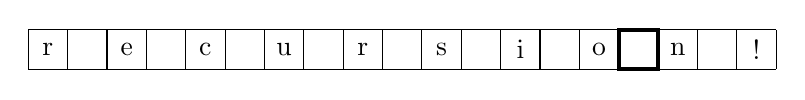
\begin{tikzpicture}
			% Specify the positions of the vertices:
			\coordinate (A0) at (0.0, 0, 0);
			\coordinate (B0) at (0.0, 0.5, 0);
			\coordinate (A1) at (0.5, 0, 0);
			\coordinate (B1) at (0.5, 0.5, 0);
			\coordinate (A2) at (1.0, 0, 0);
			\coordinate (B2) at (1.0, 0.5, 0);
			\coordinate (A3) at (1.5, 0, 0);
			\coordinate (B3) at (1.5, 0.5, 0);
			\coordinate (A4) at (2.0, 0, 0);
			\coordinate (B4) at (2.0, 0.5, 0);
			\coordinate (A5) at (2.5, 0, 0);
			\coordinate (B5) at (2.5, 0.5, 0);
			\coordinate (A6) at (3.0, 0, 0);
			\coordinate (B6) at (3.0, 0.5, 0);
			\coordinate (A7) at (3.5, 0, 0);
			\coordinate (B7) at (3.5, 0.5, 0);
			\coordinate (A8) at (4.0, 0, 0);
			\coordinate (B8) at (4.0, 0.5, 0);
			\coordinate (A9) at (4.5, 0, 0);
			\coordinate (B9) at (4.5, 0.5, 0);
			\coordinate (A10) at (5.0, 0, 0);
			\coordinate (B10) at (5.0, 0.5, 0);
			\coordinate (A11) at (5.5, 0, 0);
			\coordinate (B11) at (5.5, 0.5, 0);
			\coordinate (A12) at (6.0, 0, 0);
			\coordinate (B12) at (6.0, 0.5, 0);
			\coordinate (A13) at (6.5, 0, 0);
			\coordinate (B13) at (6.5, 0.5, 0);
			\coordinate (A14) at (7.0, 0, 0);
			\coordinate (B14) at (7.0, 0.5, 0);
			\coordinate (A15) at (7.5, 0, 0);
			\coordinate (B15) at (7.5, 0.5, 0);
			\coordinate (A16) at (8.0, 0, 0);
			\coordinate (B16) at (8.0, 0.5, 0);
			\coordinate (A17) at (8.5, 0, 0);
			\coordinate (B17) at (8.5, 0.5, 0);
			\coordinate (A18) at (9.0, 0, 0);
			\coordinate (B18) at (9.0, 0.5, 0);
			\coordinate (A19) at (9.5, 0, 0);
			\coordinate (B19) at (9.5, 0.5, 0);
			\coordinate (A20) at (10.0, 0, 0);
			\coordinate (B20) at (10.0, 0.5, 0);
			% Specify the position of the characters:
			\coordinate (C0) at(0.25, 0.25, 0);
			\node at (C0) {r};
			\coordinate (C1) at(0.75, 0.25, 0);
			\node at (C1) { };
			\coordinate (C2) at(1.25, 0.25, 0);
			\node at (C2) {e};
			\coordinate (C3) at(1.75, 0.25, 0);
			\node at (C3) { };
			\coordinate (C4) at(2.25, 0.25, 0);
			\node at (C4) {c};
			\coordinate (C5) at(2.75, 0.25, 0);
			\node at (C5) { };
			\coordinate (C6) at(3.25, 0.25, 0);
			\node at (C6) {u};
			\coordinate (C7) at(3.75, 0.25, 0);
			\node at (C7) { };
			\coordinate (C8) at(4.25, 0.25, 0);
			\node at (C8) {r};
			\coordinate (C9) at(4.75, 0.25, 0);
			\node at (C9) { };
			\coordinate (C10) at(5.25, 0.25, 0);
			\node at (C10) {s};
			\coordinate (C11) at(5.75, 0.25, 0);
			\node at (C11) { };
			\coordinate (C12) at(6.25, 0.25, 0);
			\node at (C12) {i};
			\coordinate (C13) at(6.75, 0.25, 0);
			\node at (C13) { };
			\coordinate (C14) at(7.25, 0.25, 0);
			\node at (C14) {o};
			\coordinate (C15) at(7.75, 0.25, 0);
			\node at (C15) { };
			\coordinate (C16) at(8.25, 0.25, 0);
			\node at (C16) {n};
			\coordinate (C17) at(8.75, 0.25, 0);
			\node at (C17) { };
			\coordinate (C18) at(9.25, 0.25, 0);
			\node at (C18) {!};
			% Draw vertical edges:
			\draw (B0) -- (A0);
			\draw (B1) -- (A1);
			\draw (B2) -- (A2);
			\draw (B3) -- (A3);
			\draw (B4) -- (A4);
			\draw (B5) -- (A5);
			\draw (B6) -- (A6);
			\draw (B7) -- (A7);
			\draw (B8) -- (A8);
			\draw (B9) -- (A9);
			\draw (B10) -- (A10);
			\draw (B11) -- (A11);
			\draw (B12) -- (A12);
			\draw (B13) -- (A13);
			\draw (B14) -- (A14);
			\draw (B15) -- (A15);
			\draw (B16) -- (A16);
			\draw (B17) -- (A17);
			\draw (B18) -- (A18);
			\draw (B19) -- (A19);
			\draw (B0) -- (A0);
			% Draw horizontal edges:
			\draw (A0) -- (A19);
			\draw (B0) -- (B19);
			% Draw ultra-thick grid at head's position:
			\draw[ultra thick] (B15) --(A15)-- (A16) --(B16) -- cycle;
		\end{tikzpicture}
	\end{center}
\medskip
\end{document}